\let\negmedspace\undefined
\let\negthickspace\undefined
\documentclass[a4,12pt,onecolumn]{IEEEtran}
\usepackage{amsmath,amssymb,amsfonts,amsthm}
\usepackage{algorithmic}
\usepackage{graphicx}
\usepackage{textcomp}
\usepackage{xcolor}
\usepackage{txfonts}
\usepackage{listings}
\usepackage{enumitem}
\usepackage{mathtools}
\usepackage{gensymb}
\usepackage[breaklinks=true]{hyperref}
\usepackage{tkz-euclide}
\usepackage{listings}
\usepackage{circuitikz}
\DeclareMathOperator*{\Res}{Res}
\renewcommand\thesection{\arabic{section}}
\renewcommand\thesubsection{\thesection.\arabic{subsection}}
\renewcommand\thesubsubsection{\thesubsection.\arabic{subsubsection}}
\renewcommand\thesectiondis{\arabic{section}}
\renewcommand\thesubsectiondis{\thesectiondis.\arabic{subsection}}
\renewcommand\thesubsubsectiondis{\thesubsectiondis.\arabic{subsubsection}}
\hyphenation{op-tical net-works semi-conduc-tor}
\def\inputGnumericTable{}                                
\lstset{
frame=single, 
breaklines=true,
columns=fullflexible
}
\begin{document}
\newtheorem{theorem}{Theorem}[section]
\newtheorem{problem}{Problem}
\newtheorem{proposition}{Proposition}[section]
\newtheorem{lemma}{Lemma}[section]
\newtheorem{corollary}[theorem]{Corollary}
\newtheorem{example}{Example}[section]
\newtheorem{definition}[problem]{Definition}
\newcommand{\BEQA}{\begin{eqnarray}}
\newcommand{\EEQA}{\end{eqnarray}}
\newcommand{\define}{\stackrel{\triangle}{=}}
\bibliographystyle{IEEEtran}
\providecommand{\mbf}{\mathbf}
\providecommand{\pr}[1]{\ensuremath{\Pr\left(#1\right)}}
\providecommand{\qfunc}[1]{\ensuremath{Q\left(#1\right)}}
\providecommand{\sbrak}[1]{\ensuremath{{}\left[#1\right]}}
\providecommand{\lsbrak}[1]{\ensuremath{{}\left[#1\right.}}
\providecommand{\rsbrak}[1]{\ensuremath{{}\left.#1\right]}}
\providecommand{\brak}[1]{\ensuremath{\left(#1\right)}}
\providecommand{\lbrak}[1]{\ensuremath{\left(#1\right.}}
\providecommand{\rbrak}[1]{\ensuremath{\left.#1\right)}}
\providecommand{\cbrak}[1]{\ensuremath{\left\{#1\right\}}}
\providecommand{\lcbrak}[1]{\ensuremath{\left\{#1\right.}}
\providecommand{\rcbrak}[1]{\ensuremath{\left.#1\right\}}}
\theoremstyle{remark}
\newtheorem{rem}{Remark}
\newcommand{\sgn}{\mathop{\mathrm{sgn}}}
\providecommand{\res}[1]{\Res\displaylimits_{#1}} 
\providecommand{\mtx}[1]{\mathbf{#1}}
\providecommand{\fourier}{\overset{\mathcal{F}}{ \rightleftharpoons}}
\providecommand{\system}{\overset{\mathcal{H}}{ \longleftrightarrow}}
\newcommand{\solution}{\noindent \textbf{Solution: }}
\newcommand{\cosec}{\,\text{cosec}\,}
\providecommand{\dec}[2]{\ensuremath{\overset{#1}{\underset{#2}{\gtrless}}}}
\newcommand{\myvec}[1]{\ensuremath{\begin{pmatrix}#1\end{pmatrix}}}
\newcommand{\mydet}[1]{\ensuremath{\begin{vmatrix}#1\end{vmatrix}}}
\let\vec\mathbf
\title{
\Huge\textbf{ GATE 2023 Assignment}\\
\Huge\textbf{EE1205} Signals and Systems\\
}
\large\author{Kurre Vinay\\EE23BTECH11036}
\maketitle
\bigskip
\renewcommand{\thefigure}{\theenumi}
\renewcommand{\thetable}{\theenumi}
\textbf{Question(IN 46):}
In the circuit shown ,$\omega=100\pi\text{rads/s}$, R1=R2=$2.2\Omega$ and L=$7\text{mH}$. the capacitance $\text{C}$ for which $Y_{in}$ is purely real is \marco $\text{mF}$ \\
	\vspace{0.3cm}
	\begin{center}
	\begin{circuitikz} \centering \draw 
		(0,4) to[sinusoidal voltage source, l=$V_{0}$cos($\omega$t)] (0,0)
		(0,4) to[short] (4,4)
		(4,4) to[resistor, l=$R_1$ ] (4,2)
		(4,2) to[inductor, l= $\text{L} $] (4,0) to[short ] (0,0)
		(8,4)  to[short] (4,4)
		(8,4) to[resistor, l= $R_2$] (8,2) to[capacitor,l=$\text{C}$] (8,0) to (4,0)
		;
	\end{circuitikz}
	\end{center}
\\ \hfill(GATE ST 2023)\\
\solution
 \begin{center}
\begin{tabular}{|c|c|c|}
   \hline
   variable&value&description  \\
   \hline
   $Y_{in}$ & & Admittance of circuit\\
   \hline
   $X_{L}$ & $7j\omega\Omega$ & Inductive reactance \\
   \hline
   $X_{C}$ &$\frac{-j}{\omega\text{C}}\Omega $ & Capacitive reactance \\
   \hline
   $\omega$ &$100\pi$rads/s& Angular frequency\\
   \hline
  
\end{tabular}\
\\
\caption{Table: Input Parameters}\\
\end{center}
\begin{align}
X_L&=\omega\text{L}j\\
 &=100\pi\times 7 \times 10^{-3}j \\
 &= 2.2j\Omega\\
X_C&=\frac{-j}{\omega \text{C}}\Omega\\
Y_{in}&=\frac{1}{2.2+2.2j} + \frac{1}{2.2-\frac{j}{\omega \text{C}}}\\
&=\frac{1-j}{4.4} + \frac{2.2+\frac{j}{\omega \text{C}}}{(2.2)^2+\brak{\frac{1}{\omega \text{C}}}^2}
\end{align}
According to the question given, $Y_{in}$ is purely real , so imaginary part should be equal to zero\\
\begin{align}
\frac{-1}{4.4}+\frac{\frac{1}{\omega\text{C}}}{(2.2)^2+\brak{\frac{1}{\omega\text{C}}}^2} &= 0\\
\frac{\frac{1}{\omega\text{C}}}{(2.2)^2+\brak{\frac{1}{\omega\text{C}}}^2}&=\frac{1}{4.4}\\
(2.2)^2-\frac{4.4}{\omega\text{C}}+\brak{\frac{1}{\omega\text{C}}}^2&=0\\
\brak{2.2-\frac{1}{\omega\text{C}}}^2&=0\\
\frac{1}{\omega\text{C}}&=2.2\\
\text{C}&=\frac{700}{484}\text{mF}\\
\text{C}&=1.446281\text{mF}
\end{align}
The capacitance of capacitor $\text{C}$ is 1.45$\text{mF}$
\begin{figure}[ht!]
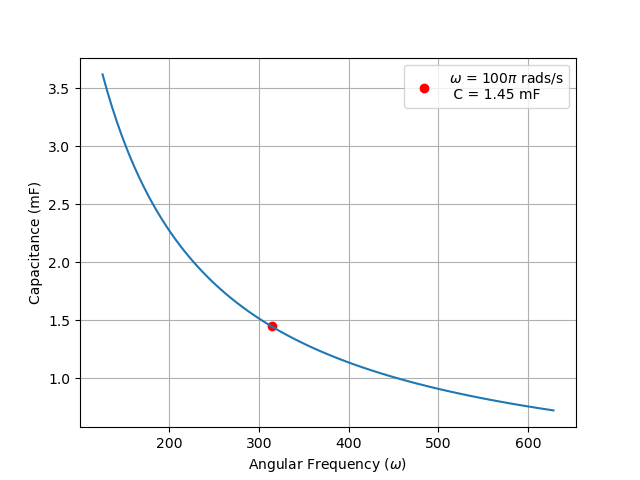
\includegraphics[width=\columnwidth]{fig/fig3.png}
\caption{Graph of Capacitance($\text{mF}$) vs Angular Frequency($\omega$)}
\end{figure}
\end{document}
